\jxhj{%教学后记
	}
\skrq{%授课日期
	2017年12月7日 4-5节}
\ktmq{%课题名称
	 长度补偿应用}
\jxmb{%教学目标,每行前面要加 \item
	\item 掌握Fanuc上的长度补偿指令;
	\item 掌握Fanuc长度补偿的执行过程;
	\item 掌握Fanuc长度补偿的编程;
	\item 会进行各种长度补偿的使用。}
\jxzd{%教学重点,每行前面要加 \item
	\item Fanuc长度补偿的执行过程;
	\item 长度补偿的编程。 }
\jxnd{%教学难点,每行前面要加 \item
	\item 进行各种长度补偿的使用。 }
\jjff{%教学方法
	通过讲述、举例、演示法来说明;}

\makeshouye %制作教案首页

%%%%教学内容
\subsection{组织教学}
\begin{enumerate}[\hspace{2em}1、]
	\item 集中学生注意力;
	\item 清查学生人数;
	\item 维持课堂纪律;
\end{enumerate}

\subsection{复习导入及主要内容}
\begin{enumerate}[1、]
\item 长度补偿概述;
\item 长度补偿方向的确定;
\item 长度补偿值的确定;
\item 换刀指令。
\end{enumerate}

\subsection{教学内容及过程}
\subsubsection{长度补偿的执行过程}
	
	过程一:
	
	补偿时,先进行补偿,后进行定位
	
	取消时,先取消补偿,后进行定位
	
	注意安全问题:
	
	程序启动前,要求刀具工件表面有足够的补偿空间。
	
	取消之前,先提刀,保证有足够的取消空间
	
	过程二:
	
	补偿时,补偿与定位计算,直接一次移动到位。
	
	取消时,取消与定位计算,直接一次移动到位。
	
	这种方法使用安全
	
\subsubsection{安全使用长度补偿}
	
	1、程序启动前,要求刀具到工件表面的距离大于最大的刀具长度补偿。
	
	2、程序中取消刀补,要求先提刀到一个较高的位置,在取消。
	
	即使用及取消刀具长度补偿要有足够的空间。
	
	3、编程要求
	
	G43G1Z150.H1 (Z150大于最大的刀具半径补偿)
	
	……
	
	G1Z100.F2000 (提刀到一个较高的位置)
	
	G49G1Z150.
	
	……
	
\subsubsection{三种补偿值的比较}
	
	1、相对长度:
	
	容易理解,但基准刀攷变时,所有的补偿要重新设置,
	
	补偿值有正有负,为正时不安全。
	
	用基准刀对刀,对刀方便。
	
	2、绝对长度:
	
	使用刀具的绝对长度,补偿值不变,补偿值始终为正,使用不太安全
	。对刀要考虑刀具的长度,
	
	3、空间移动距离
	
	即在绝对长度的基础上,把补偿值变换为负值。
	方法,把坐标系往上提高一个距离,刀具向负方向补偿一个距离。
	
\subsubsection{编程实例}
	
	在数控机床上加工如图所示的零件,试按加工中心机床进行零件的工艺分析及程序的编写。
	
	综合加工,如图9-5所示。毛坯:80*80*45。要求:
	
	(1)面铣:保证厚度为44 
	     
	(2)轮廓铣:粗/精加工(内凸台高15mm、外凸台高15mm)    
	  
	(3)型腔铣:粗/精加工(矩形深5mm,圆形深10mm) 
	    
	(4)孔加工:$\varnothing $8H7(深25mm)
	
	刀具:面铣$\varnothing $80         粗加工$\varnothing $16、$\varnothing $12   
	   
	精加工$\varnothing $8        孔$\varnothing $5、$\varnothing $7.8   $\varnothing $8H7
	
	\begin{figure}[h]
		\centering
		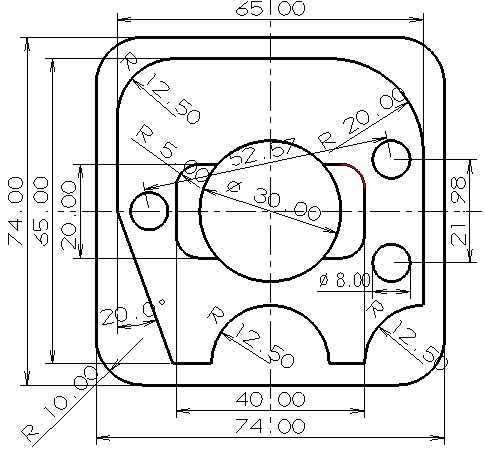
\includegraphics[width=0.7\linewidth]{data/image/25-1}
		\caption{编程实例}
		\label{fig:25-1}
	\end{figure}
	
	1、图形分析
	
	2、坐标系及装夹
	
	3、刀具及工序标
	
	A 铣上表面  $\varnothing$80面铣刀 T1H1 S400 F200 
	
	B 粗铣外形  $\varnothing$16立铣刀 T2H2 S500 F200 D1=8.5
	
	C 粗铣槽    $\varnothing$12 立铣刀 T3H3 S500 F200 D2=6.5
	
	D 精加工    $\varnothing$8立铣刀  T4H4  S800 F100 D3=6.2
	
	E 钻中心空  $\varnothing$3中心钻   T5H5 S1000 F60
	
	F 钻孔     $\varnothing$7.8麻花钻 T6H6 S500  F80
	
	H 铰孔      $\varnothing$8H7机用铰刀  T7H7 S300 F30
	
	
	4、参考程序
	\begin{lstlisting}
	O1
	G28G91ZO
	T1M6
	M98P2 (铣平面)
	G28G91Z0
	T2M6
	M98P3 (铣方)
	M98P4  (铣外形)
	G28G91Z0
	T3M6
	M98P5  (铣槽)
\end{lstlisting}

\subsection{课堂小结}
\begin{enumerate}[1、]
\item Fanuc长度补偿的执行过程;
\item 安全使用长度补偿;
\item 三种补偿值的比较;
\item 编程实例。
\end{enumerate}

\vfill
\subsection{布置作业}
\begin{enumerate}[1、]
	\item 综合习题一。
\end{enumerate}
\vfill